%% The first command in your LaTeX source must be the \documentclass command.
%%
%% Options:
%% twocolumn : Two column layout.
%% hf: enable header and footer.
\documentclass[
% twocolumn,
% hf,
]{ceurart}

%%
%% One can fix some overfulls
% \sloppy

%%
%% Minted listings support 
%% Need pygment <http://pygments.org/> <http://pypi.python.org/pypi/Pygments>
\usepackage{minted}
\usepackage{tikz}
\usepackage{subcaption}
% \usepackage{biblatex}
%% auto break lines
\setminted{breaklines=true}


\usetikzlibrary{shapes.geometric, arrows, positioning}


%

\tikzstyle{startstop} = [rectangle, rounded corners, minimum width=3cm, minimum height=1cm, text centered, draw=black, fill=gray!30]
\tikzstyle{process} = [rectangle, minimum width=3cm, minimum height=1cm, text centered, draw=black, fill=blue!20]
\tikzstyle{annotation} = [rectangle, text width=6cm, align=left, draw=black, fill=yellow!20, rounded corners, minimum height=2.5cm]
\tikzstyle{arrow} = [thick,->,>=stealth]

%\tikzstyle{startstop} = [rectangle, rounded corners, minimum width=3cm, minimum height=1cm, text centered, draw=black, fill=gray!30]
%\tikzstyle{process} = [rectangle, minimum width=3cm, minimum height=1cm, text centered, draw=black, fill=blue!20]
%\tikzstyle{annotation} = [rectangle, text width=8cm, align=left, draw=black, fill=yellow!20, rounded corners, minimum height=2.5cm]
%\tikzstyle{arrow} = [thick,->,>=stealth]


%%
%% end of the preamble, start of the body of the document source.
\begin{document}

%%
%% Rights management information.
%% CC-BY is default license.

    \copyrightyear{2024}
    \copyrightclause{Copyright for this paper by its authors.
    Use permitted under Creative Commons License Attribution 4.0
    International (CC BY 4.0).}

%%
%% This command is for the conference information

    \conference{RuleML+RR'24: Companion Proceedings of the 8th International Joint Conference on Rules and Reasoning,
        September 16--22, 2024, Bucharest, Romania}


%%
%% The "title" command
    \title {
        Optimising Hierarchical Demand Forecasting with Explainable AI: Insights into Key Drivers
    }

%%
%% The "author" command and its associated commands are used to define
%% the authors and their affiliations.
    \author{M\'{a}ty\'{a}s Kuti-Kresz\'{a}cs}[%
        orcid=0009-0004-4997-2000,
        email=matyas.kuti@ubbcluj.ro,
        url=https://www.linkedin.com/in/kkmatyas/,
    ]

    \address{
%Babeș-Bolyai University, Cluj-Napoca
        Babe\c{s}-Bolyai University, Cluj-Napoca
    }


%%
%% The abstract is a short summary of the work to be presented in the
%% article.
    \begin{abstract}
%        A clear and well-documented \LaTeX{} document
%        is presented as an
%        article formatted for publication by CEUR-WS in a conference
%        proceedings. Based on the ``ceurart'' document class, this article
%        presents and explains many of the common variations, as well as many
%        of the formatting elements an author may use in the preparation of
%        the documentation of their work.
%        \textcolor{red}{
%            Demand forecasting is a prediction problem that aims to estimate future needs based on historical data.
%            In order to better understand the decision-making process of hierarchical demand forecasting models,
%            we propose a method to apply SHAP values to the forecasting model, aiming to identify the key drivers of the forecast. This method can help to understand the impact of price changes, promotional activities, and resource planning on forecasting accuracy. In our current work, we use a real-world dataset to evaluate the proposed methods. We use XAI(Explainable AI) techniques to identify key features and analyze their impact on the forecasts.
%        }
        Demand forecasting is a prediction problem that aims to estimate future needs based on historical data.
        It serves as the basis for optimal decision making in multiple areas of value chains such as manufacturing, logistics, and retail.
        It is particularly important in demand forecasting models where demand drivers like price, promotions, and resource planning can help companies optimise pricing, promotional activities, resource planning, and inventory planning.
        Our goal is to identify applicable feature importance techniques to hierarchical forecasting problems by providing insights into feature importance and the underlying decision-making process and helping to understand the model's reasoning.
        We propose applying SHAP values to a forecasting model while using part of a real-world dataset.
        The results will provide insight into the key drivers of the forecast and help to understand the impact of the features
        on the decisions made by the model.
    \end{abstract}

    \maketitle
%
%\textcolor{red}{ %TODO: Add the following sections
%The submission should cover the following aspects:
%\begin{itemize}
%    \item (Identified some, but if it's relevant) The identification of a significant problem in a research field relevant to RuleML+RR 2024.
%    \item (Done) An outline of the current knowledge in the problem’s domain, as well as an overview of existing solutions.
%    \item (Review) A clear formulation of the research question and motivation.
%    \item (Results added not described) A presentation of (possibly preliminary) ideas, the proposed approach, and the results achieved so far.
%    \item (Review)A sketch of the applied research methodology and its positioning in the field.
%    \item (Expected contribution:done)A description of the student’s contribution to the research.
%    \item (TODO:)A discussion of how the suggested solution is different, new, or better as compared to the state of the art.
%    \item (Done)A research plan and the potential achievements.
%\end{itemize}
%}

%The accepted DC papers will be presented to an interested audience and will be discussed with a panel of senior researchers from academia and the industry. Students will present their work through brief oral presentations during a dedicated session of RuleML+RR 2024.





    \section{Introduction}\label{sec:introduction}
%\textcolor{blue}{
%%Introduction
%\begin{itemize}
%    \item Background: Importance of demand forecasting, machine learning, and hierarchical forecasting.
%    \item Problem Statement: Challenges in understanding the rules and reasoning in hierarchical demand forecasting models.
%    \item Objectives: Apply XAI to identify and analyze feature importance and the underlying rules in hierarchical models.
%    \item Significance: Enhanced transparency, reasoning, and improved forecasting accuracy across hierarchical levels.
%\end{itemize}
%}
%\textcolor{black}

%Demand forecasting is a critical aspect of business operations, helping organizations make informed decisions about production, inventory, and resource allocation. Machine learning models have become increasingly popular for demand forecasting due to their ability to capture complex patterns in historical data. Hierarchical forecasting is a specialized approach that considers the hierarchical structure of the data, such as product categories, geographical regions, or time periods, to improve forecasting accuracy. However, understanding the rules and reasoning behind these models can be challenging, especially when dealing with large and complex datasets.

Demand forecasting became really important for businesses and serves as the basis for optimal decision making in multiple areas in value chains such as manufacturing, logistics, and retail.
%Given that the production and distribution of goods are influenced by the demand, accurate demand forecasting is crucial for companies to optimize their inventory levels, production planning, and resource allocation.
By having multiple products, manufacturing locations, sales channels, and geographical regions, demand forecasting can be complex and hierarchical in nature.

However, the problem can be formulated as a regression problem, with the aim of predicting the future demand based on historical data.
This regression problem can be solved using machine learning models such as random forests, gradient boosting, and neural networks.
Unfortunately, these models are considered black boxes and their predictions are hard to interpret.
This is where explainable AI (XAI) techniques come into play, providing insights into the model's decision-making process and helping to understand the underlying rules and reasoning behind the predictions.

One of the most fundamental methods for understanding a model's reasoning is feature importance or attribution, which allows identifying key contributor factors to the model's predictions.
This is especially important in demand forecasting models, where demand drivers, such as price, promotions, weather, holidays, and economic indicators, can influence demand.
Understanding these drivers can help companies optimize pricing, promotional activities, resource planning, and inventory management.

Our goal is to identify applicable feature importance techniques to demand forecasting models, aiming to discover key features contributing to the decisions and explain the model's reasoning at different levels.
The significance of our research is to improve the reasoning and transparency of multiseries and hierarchical demand forecasting models by providing insights into feature importance and the underlying rules at various levels.
The methods employed are expected to be used not only in demand forecasting, but also in other grouped and hierarchical forecasting problems in different domains.


\subsection{Research Questions}\label{sec:research_questions}

The gap identified in the literature is the lack of studies that apply feature importance techniques to multiseries models
for hierarchical demand forecasting problems and analyse the underlying decision drivers at different levels.
Other studies focused on the representation of the explanation for sales forecasting models, but not on the explanation methods themselves\cite{fahse2022explanation}.
Our research questions are:
\begin{itemize}
    \item \textbf{RQ1:} Can existing feature importance techniques be applied to multi-series and hierarchical models to identify key features and explain the underlying decision factors?
%    \item \textbf{RQ1:} How can feature importance techniques be applied to multi-series and hierarchical models
    \item \textbf{RQ2:} How feature importance can be translated to different hierarchical levels?
    \item \textbf{RQ3:} How do these methods perform when applied to real-world datasets?
    \item \textbf{RQ4:} How can the results be visualised and interpreted?
    \item \textbf{RQ5:} What methods are most effective in this context?
\end{itemize}

In our current work, we partially address RQ1 and RQ2 by proposing a method to apply SHAP values to a LightGBM model
used for forecasting hierarchical time-series data.
Furthermore, we make progress on RQ3 using part of a real-world dataset; however, evaluation is still pending.
Last but not least, we address RQ4 by visualising the results in a way that can be interpreted by the user.
RQ5 is still open and will be addressed in future work.



%This way, the demand forecasting models can help companies to optimize their inventory levels, production planning, and resource allocation.
%machine learning models are being used more and more compared to traditional statistical models due to their ability to capture complex patterns in historical data while being more flexible to adapt various data.

%is a specialized approach that considers the hierarchical structure of the data, such as product categories, geographical regions, or time periods, to improve forecasting accuracy. However, understanding the rules and reasoning behind these models can be challenging, especially when dealing with large and complex datasets.

%
%
%%Literature Review
%\begin{itemize}
%    \item  Demand Forecasting Methods: Machine learning models used.
%    \item Multi-series, multivariate and hierarchical forecasting: Concept and importance.
%    \item Global and grouped feature importance: Techniques for understanding feature importance at different levels.
%    \item Rules and Reasoning in AI: Understanding model decisions.
%    \item Existing Research: Studies on feature importance, hierarchical forecasting, and XAI in model reasoning.
%    \item Research Gaps: Need for XAI application in hierarchical forecasting.
%\end{itemize}

%Demand Forecasting Methods: Machine learning models used.
%\color{red}
%Demand forecasting is a critical aspect of business operations, helping organizations make informed decisions about production, inventory, and resource allocation.
%Machine learning models have become increasingly popular for demand forecasting due to their ability to capture complex patterns in historical data.
%Hierarchical forecasting is a specialized approach that considers the hierarchical structure of the data, such as product categories, geographical regions, or time periods, to improve forecasting accuracy.
%However, understanding the rules and reasoning behind these models can be challenging, especially when dealing with large and complex datasets.
%Explainable AI (XAI) techniques provide insights into the model's decision-making process and help understand the underlying rules and reasoning behind the predictions.
%Our objective is to apply feature importance techniques from XAI to hierarchical demand forecasting models, aiming to identify key features contributing to the decisions and explain the model's reasoning at different hierarchical levels.
%We aim to tackle global and grouped feature importances as we are interested in understandign the importance of features at different levels of the hierarchy.
%Global feauture importance techniques like permutation fearure importance to understand the importance of features at the global level while local  SHAP importances can be used as grouped feature importances(cohort) techniques can be used to understand the importance of features at the group level.
%\color{black}


\section{Literature review}\label{sec:literature_review}


%\textbf{Forecasting ensemble models}
%\subsection{Demand Forecasting with machine learning} \label{subsec:demand-forecasting-with-machine-learning}
%Demand forecasting is a prediction problem that aims to estimate future needs based on historical data.
%Statistical forecasting methods such as ARIMA\cite{jamal_fattah_forecasting_2018,ingle2021demand} and exponential smoothing \cite{ingle2021demand} have been widely used in demand forecasting.
%However, they have limitations in intermittent multi-series and hierarchical forecasting, where machine learning models have shown better performance\cite{spiliotis2022comparison}.
%An important aspect also is that there may be multiple exogenous variables so-called demand drivers\cite{vandeput2023demand} that can influence the demand.
%Internal factors such as price, promotions, and external factors like weather, holidays, and economic indicators can be considered as demand drivers.
%These can be used as features in machine learning models to improve forecast accuracy.
%
%Machine learning models such as tree ensembles and neural networks have been successfully applied to demand forecasting tasks\cite{spiliotis2022comparison}.
%Ensemble models in general can be homogeneous with individual models of the same type or heterogeneous with models of different types.
%We considered only homogeneous ensemble tree models because of the applicability of some model-specific explanation methods.
%To build tree ensembles, bagging methods such as random forest\cite{leo_breiman_random_2001} can be used, which trains multiple decision trees on different subsets of the data, and the final prediction is the average of the predictions of the individual models.
%In addition, boosting methods such as Gradient Boosting Machines (GBM) \cite{jerome_h_friedman_greedy_2001}, XGBoost \cite{tianqi_chen_xgboost_2016}, and LightGBM \cite{guolin_ke_highly_2017}, which train models sequentially on the residuals of the previous model, in this case using the sum of individual predictions.
%In a notable forecasting competition \cite{makridakis_m5_2022}, a LightGBM model was the winner and secured four of the top five positions.
%
%\subsection{Forecasting techniques} \label{subsec:forecasting-techniques}
%Forecasting techniques can be divided into single-series or multi-series forecasting from the perspective of the model's input.
%Single-series forecasting refers to the prediction of a single time series, while multiseries forecasting involves the prediction of multiple time series, with the same global model\cite{joachim2023demand}.
%These series can be related to each other, such as sales of different products, or they can be independent, such as sales in different regions; therefore, it is important to consider the hierarchical structure of the data.
%
%Hierarchical forecasting refers to the prediction of multiple time series that are related to each other in a hierarchical structure\cite{hyndman2018forecasting}.
%It can be tackled with different single-level approaches, such as bottom-up, top-down, or middle-out\cite{hyndman2018forecasting}.
%The top-down approach would involve a single series model for the total demand and then disaggregating it to the lower levels.
%The middle-out and bottom-up approach would involve a multiseries model.
%Grouped time-series forecasting is a special case of hierarchical forecasting, where the series are aggregated based on attributes such as product type, region, or sales channel.
%
%\cite{vandeput2023demand} suggests three major hierarchies in demand forecasting: product hierarchy, geographical hierarchy, and time hierarchy.
%The product hierarchy refers to the categorisation of products according to their attributes, such as product type, brand, or category.
%The geographic hierarchy involves the division of sales regions based on geographic attributes, such as country, state, or city down to the point of sale.
%Time hierarchy refers to the temporal structure of the data, such as year, month, week, day, and hour.

%\subsection{Feature importance} \label{subsec:feature-importance-in-tree-ensemble-models}
%Feature importance (FI) or feature attribution is considered an interpretation method resulting in a summary statistic that assigns a score to each input feature \cite{molnar2022}.
%Depending on their scope, the FI methods can be global or local \cite{Guidotti2018,molnar2022}.
%The global feature importance (GFI) or model feature attribution methods explain the contribution of features to overall predictions, while the local FI quantifies feature contributions to specific predictions \cite{molnar2022}.
%Although related, GFI methods differ from feature selection, which identifies irrelevant features before training.
%GFI methods can be model-specific, which are limited to specific model types, while model-agnostic ones are applicable independent of the model type\cite{molnar2022}.
%Another categorisation of FI methods is given by how it is calculated, in which case the importance can be based on the model's structure, while the other approach relies on a dataset.
%
%Among the model-agnostic methods, one of the most common is permutation feature importance (PFI) which was proposed to measure FI in random forests\cite{Breiman2001}.
%It is a model-agnostic, data-dependent method that measures the decrease in the model's performance when the features are permuted.
%The PFI can be calculated using different metrics such as the mean squared error (MSE), the mean absolute error (MAE), or the coefficient of determination ($R^2$).
%PFI also has limitations, as it is sensitive to over- and underfitting\cite{molnar2020limitations}, in which case the FI differs on training and test data, so the use of both datasets can be beneficial.
%In addition, another flaw of the PFI method is that it can generate cases in which the model does not have training data\cite{Molnar_2020_pitfalls,giles_hooker_unrestricted_2021},
%but other methods were proposed to overcome this\cite{ian_covert_understanding_2020, kristin_blesch_conditional_2023}.
%% todo include conditional PFI
%
%SHAP(SHapley Additive exPlanation)\cite{scott_lundberg_unified_2017} values contribute local explanation for individual predictions, but aggregates of it are useful to assess the importance of global features.
%For example, the mean absolute SHAP values quantify the importance of the feature regardless of the direction of the impact on the prediction.
%There are different algorithms for approximation from which Kernel SHAP\cite{scott_lundberg_unified_2017} is one that is model-agnostic.
%TShap \cite{vikas_c_raykar_tsshap_2023} is a method for estimating SHAP values for time series data, but it uses a surrogate model, so it gives the FI of the surrogate.
%Another related method is SAGE \emph{(Shapley additive global importance)} \cite{ian_covert_understanding_2020}, which estimates the contribution of each feature to the model's performance.
%
%Tree specific GFI methods are gain-based importance values which were already introduced with decision trees \cite{gordon_classification_1984}
%It measures of the reduction in mean average error(MAE) made by the decisions based on the respective feature.
%Another measure is the split-based importance\cite{tianqi_chen_xgboost_2016} refers to the number of decisions made by the model based on a feature.
%The previously presented SHAP also has a tree model-specific solution for approximation, called TreeSHAP \cite{scott_lundberg_local_2020}
%
%%\subsection{Triad of model interpretability}
%%The triad of model interpretability consists of model transparency, model trust, and model understanding\cite{molnar2022}.
%
%\subsection{Explainability in forecasting}\label{subsec:explainability-in-forecasting}
%The number of publications on forecasting explainability is limited.
%\cite{fahse2022explanation} tackled the presentation of explanations for sales forecasting models, but not the explanation methods themselves.
%\cite{Saluja_2021} used SHAP values to explain the prediction of a time series model but on local level and not global level.
%Skforecast~cite{joachim2023demand} library extracts model specific global feature importance from tree ensemble models.
%The work is focused on either global feature importance or local feature contribution without considering the multi-series and hierarchical structure of the data.
%
%\subsection{Feature importance as a basis for model reasoning}\label{subsec:feature-importance-as-basis-for-model-reasoning}
%Feature importance methods can provide insight into the model's decision-making process and help to understand the underlying rules and reasoning behind the predictions.
%By including demand drivers as features in the model, the feature importance methods can help to identify the key drivers of demand.
%For external factors such as weather, holidays, and economic indicators, the importance of the characteristics can help to understand their impact on demand.
%Through internal factors like price, promotions, the feature importance can help to understand post-promotion effects and the impact of price changes on the demand\cite{vandeput2023demand}.
%Knowing the influence of internal factors can help to optimize pricing strategies and promotional activities.
%However, causation and correlation are different concepts, and the feature importance methods can only provide correlation;
%therefore, the identified key features should be further analyzed to understand the causation\cite{Breiman2001}



%\subsection{Research Gaps}
%The literature review revealed a gap in the application of feature importance techniques to multi-series models for hierarchical demand forecasting problems.
%The studies focused on the presentation of explanations for sales forecasting models but not on the explanation methods themselves.
%Our research aims to address this gap by applying feature importance techniques to hierarchical models and analyzing the underlying decision drivers at different levels.


%Research Questions:
%\begin{itemize}
%\item How can XAI techniques be applied to hierarchical models to identify key features and explain the underlying rules?
%\item What are the differences in feature importance and model reasoning at various hierarchical levels?
%\item How does understanding the rules and reasoning improve forecasting accuracy?
%\end{itemize}


%%! Author =
%
%
%\section{Introduction}
%
%\begin{itemize}
%\item Background: Importance of demand forecasting, the role of machine learning, and the concept of hierarchical forecasting.
%\item Problem Statement: Challenges in achieving interpretability and accuracy in hierarchical demand forecasting models.
%\item Objectives: To apply explainable AI methods to identify and analyze feature importance in hierarchical demand forecasting models.
%\item Significance: Improved transparency and trust in machine learning models, better feature selection, and enhanced forecasting accuracy across hierarchical levels.
%\end{itemize}
%Literature Review:
%
%\begin{itemize}
%\item Demand Forecasting with Machine Learning: Overview of machine learning techniques (e.g., decision trees, random forests, gradient boosting) used in demand forecasting.
%\item Hierarchical Forecasting: Explanation of hierarchical forecasting, its importance, and current methods.
%\item Explainable AI (XAI) Techniques: Review of XAI methods such as SHAP (SHapley Additive exPlanations), LIME (Local Interpretable Model-agnostic Explanations), and feature importance scores.
%\item Existing Research: Discussion of existing studies on feature importance and hierarchical forecasting.
%\item Research Gaps: Identified gaps in applying XAI for feature importance in hierarchical demand forecasting models.
%\end{itemize}
%
%
%Research Questions or Hypotheses:
%
%\begin{itemize}
%\item Research Questions:\begin{enumerate}
%\item How can explainable AI techniques be applied to hierarchical demand forecasting models to identify key features?
%\item What are the differences in feature importance at different hierarchical levels?
%\item How does understanding feature importance at various levels improve overall forecasting accuracy?
%\end{enumerate}
%
%\end{itemize}
%
%Hypotheses:
%\begin{enumerate}
%\item Explainable AI methods can provide clear and actionable insights into feature importance across hierarchical levels.
%\item Identifying key features at different levels enhances the accuracy and reliability of hierarchical demand forecasts.
%\end{enumerate}
%
%
%

%\include

    \section{Methodology} \label{sec:methodology_preliminary_results}

%\textcolor{blue}{
%Methodology:
%\begin{itemize}
%    \item Research Design:
%    \item Data Collection: Hierarchical datasets (e.g., sales data, economic indicators).
%    \item Methods: Implementing hierarchical models, applying XAI techniques, analyzing feature importance and reasoning.
%    \item Evaluation: Accuracy metrics and interpretability assessment.
%\end{itemize}
%}

Our preliminary research focusses on the methodological aspects of applying feature importance techniques to hierarchical forecasting models.
This includes adaptation of existing methods, but also tool development to support the analysis of hierarchical forecasting models.
Later we plan to conduct an empirical study to evaluate the methods on real-world datasets.

Our initial research design\ref{fig:research_design} includes the following steps:
\begin{itemize}
    \item Data collection: identify datasets with hierarchical time series data describing sales/demand for multiple product categories and regions with exogenous variables.
    \item Tool evaluation: assess the applicability of existing libraries for hierarchical forecasting and XAI techniques.
    \item Model implementation: we build global models that consider multiple series and exogenous variables.
    \item Feature importance analysis: We apply model attribution methods and aggregation and decomposition techniques to identify key features and analyze their impact on the forecast.
    \item Model reasoning: analyze the feature contributions to forecast and identify underlying rules on different levels of the hierarchy.
\end{itemize}


\begin{figure}
    \centering
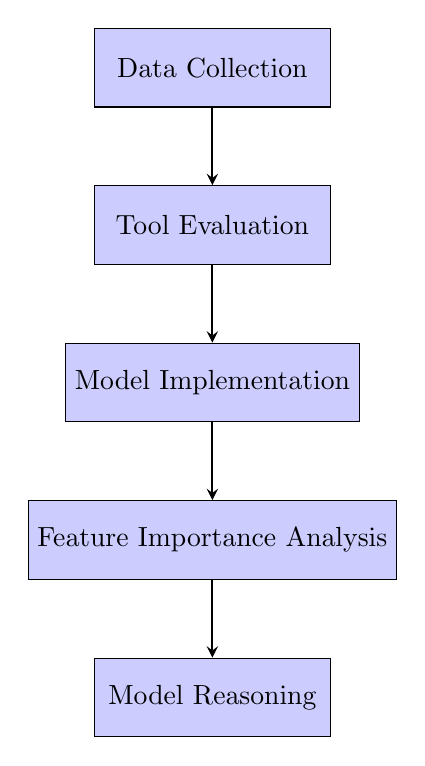
\begin{tikzpicture}[node distance=2cm]

%\node (start) [startstop] {Start};
\node (data) [process] {Data Collection};
\node (tool) [process, below of=data] {Tool Evaluation};
\node (model) [process, below of=tool] {Model Implementation};
\node (importance) [process, below of=model] {Feature Importance Analysis};
\node (reasoning) [process, below of=importance] {Model Reasoning};
%\node (stop) [startstop, below of=reasoning] {End};

%\draw [arrow] (start) -- (data);
\draw [arrow] (data) -- (tool);
\draw [arrow] (tool) -- (model);
\draw [arrow] (model) -- (importance);
\draw [arrow] (importance) -- (reasoning);
%\draw [arrow] (reasoning) -- (stop);

% Annotations
%\node [annotation, right=3cm of data.east, anchor=west] (dataann) {
%    \begin{itemize}
%        \item Find hierarchical time series data.
%        \item Include sales/demand across categories and regions.
%        \item Add relevant exogenous variables.
%    \end{itemize}
%};
%
%\node [annotation, right=3cm of model.east, anchor=west] (modelann) {
%    \begin{itemize}
%        \item Build global models for multiple time series.
%        \item Integrate exogenous variables.
%    \end{itemize}
%};
%
%\node [annotation, right=3cm of importance.east, anchor=west] (importanceann) {
%    \begin{itemize}
%        \item Determine feature importance.
%        \item Use aggregation and decomposition.
%        \item Assess feature impact on forecasts.
%    \end{itemize}
%};
%
%\node [annotation, right=3cm of reasoning.east, anchor=west] (reasoningann) {
%    \begin{itemize}
%        \item Analyze feature contributions.
%        \item Discover rules at different hierarchy levels.
%    \end{itemize}
%};
\end{tikzpicture}
\caption{Research design} \label{fig:research_design}
\end{figure}





%The research design includes the following steps:
%\begin{itemize}
%    \item Data collection: we will use datasets with hierarchical time series data describing sales/demand for multiple product categories and regions.
%    \item Model implementation: we build global models that consider multiple series and exogenous variables. The ML models include decision trees, random forests, and gradient boosting.
%    \item Feature importance analysis: we apply model attribution methods such as PFIs, SHAP and SAGE to identify key features and analyze their impact on the forecast.
%    \item Model reasoning: analyze the feature contributions to forecast and identify the underlying rules.
%\end{itemize}

\subsection{Data collection and preprocessing}\label{subsec:data-collection-and-preprocessing}
%
%To model the hierarchical impact of features on forecasting, we must use datasets with multiple series and exogenous variables that represent demand drivers.
%There are multiple open sales data sets available; however, there are just a few, such as the M5 competition\citep{makridakis_m5_2022} and the Kaggle datasets\cite{favorita-sales}.
%For our initial exploration, we sampled M5 competition\citep{makridakis_m5_2022} dataset, which includes sales data for multiple product categories and regions.
%The dataset contains daily sales information for 3049 products in 10 stores over 5 years.
%For our analysis, we identified three products that have similar sales patterns and are sold in two states and five stores.
%As products are from the same category and department, the hierarchy at the product level was not considered.
%The reason for this filtering is to reduce the complexity of the model and to focus on the feature importance analysis.
%The selected products are FOODS\_3\_586, FOODS\_3\_080, and FOODS\_3\_555 and are sold in three states of Texas (TX), Wisconsin (WI).
%The total sales data for these products are shown in Figure \ref{fig:product_sales}.
%Our hierarchical structure is shown in Figure \ref{fig:hierarchical_structure}.
%It should be mentioned that the hierarchical structure can be inverted, meaning that the products can be at the top level and the stores at the bottom level,
%so technically our data set is grouped time series data.

\begin{figure}
    \centering
    \includegraphics[width=0.8\linewidth]{sections/img/product_sales}
    \centering
    \caption{Total weekly sales for the chosen products}
    \label{fig:product_sales}
\end{figure}


%The sales we aggregated the data at the weekly level.
%\begin{itemize}
%    \item Aggregating data at the weekly level.
%    \item Splitting data into training and test sets.
%\end{itemize}


\begin{figure}
    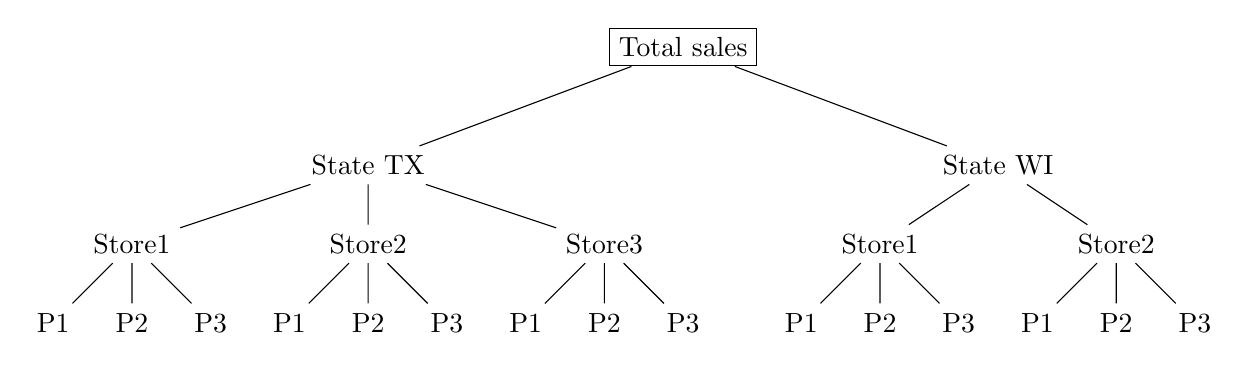
\begin{tikzpicture}
    [level 1/.style={sibling distance=80mm, level distance=15mm},
        level 2/.style={sibling distance=30mm, level distance=10mm},
        level 3/.style={sibling distance=10mm, level distance=10mm}]
        \node[rectangle,draw] {Total sales}
        child {node {State TX}
        child {node {Store1}
        child {node {P1}}
        child {node {P2}}
        child {node {P3}}
        }
        child {node {Store2}
        child {node {P1}}
        child {node {P2}}
        child {node {P3}}
        }
        child {node {Store3}
        child {node {P1}}
        child {node {P2}}
        child {node {P3}}
        }
        }
        child {node {State WI}
        child {node {Store1}
        child {node {P1}}
        child {node {P2}}
        child {node {P3}}
        }
        child {node {Store2}
        child {node {P1}}
        child {node {P2}}
        child {node {P3}}
        }
        };
    \end{tikzpicture}
    \caption{Hierarchical structure of product sales data (P1-3 = Product1-3)} \label{fig:hierarchical_structure}
\end{figure}

Data preprocessing two main parts: preparing the sales data and the exogenous variables.
Sales data were aggregated at the weekly level.
The weeks at the beginning and end of the data set were removed to have a consistent time period.
As features, lagged sales data was included to capture the temporal dependencies.
The exogenous variables were related to pricing and calendar events.
The selling price was already aggregated at the weekly level for each store and product.
Calendar events included whether a day was a holiday, had special events, and if it was a SNAP (Supplemental Nutrition Assistance Programme) day in a respective state.
To include these variables in some way, they were counted for each week and state.
In addition, the week of the year was included as a feature to capture seasonality.
The data were split into training and test sets, and the last complete year(2015) was used to test the model.
The structure of the data sales data is shown in Table \ref{tab:data_structure} and the exogenous variables in Table \ref{tab:exog_data_structure}.


%\end{table}

\begin{table}
    \centering
    \begin{resizebox}{\linewidth}{!}

        \begin{tabular}{
            |p{0.15\textwidth} % feature name
            |p{0.1\textwidth}  % feature type
            |p{0.75\textwidth}  % feature description
            |}
            \hline
            Feature name  & Type   & Description                                                                                         \\
            \hline
            week\_date    & date   & Starting date of week used for aggregation                                                          \\
            \hline
            week          & int    & Week number of the year                                                                             \\
            \hline
            series\_id    & string & Unique identifier for the series made of state+store+product combination,  representing the hierarchy \\
            \hline
            sales         & float  & Total sales for the week                                                                            \\
            \hline
            lag\_\emph{n} & float  & Sales from the previous \emph{n} weeks                                                              \\
            \hline
        \end{tabular}%
    \end{resizebox}
    \caption{ Sales data structure}
    \label{tab:data_structure}
\end{table}


\begin{table}
    \begin{tabular}{
        |p{0.15\textwidth} % feature name
        |p{0.1\textwidth}  % feature type
        |p{0.75\textwidth}  % feature description
        |}
        \hline
        Feature name    & Type   & Description                                                                                          \\
        \hline
        week\_date      & date   & Starting date of week used for aggregation                                                           \\
        \hline
        week\_of\_year  & int    & Week number of the year                                                                              \\
        \hline
        series\_id      & string & Unique identifier for the series made of state+store+product combination, representing the hierarchy \\
        \hline
        sell\_price     & float  & Selling price for the week for                                                                       \\
        \hline
        num\_of\_events & int    & The number of special events and holidays in the week                                                \\
        \hline
        snap\_days      & int    & Number of SNAP days in the week                                                                      \\
        \hline
    \end{tabular}
    \caption{Exogenous variables}
    \label{tab:exog_data_structure}
\end{table}

%\subsection{Model implementation}\label{subsec:model-implementation}
%The modelling approach is to build a single global on all series and exogenous variables for bottom-up aggregation.
%For creating forecast models, the skforecast\cite{skforecast} library was used.
%The base model for hierarchical forecasting was LightGBM~\cite{guolin_ke_highly_2017}
% due to its efficiency and also because of its widespread usage in the M5 competition in this data set\cite{makridakis_m5_2022}.
%Other ensemble models such as Random Forest or Gradient Boosting Machines could be used as well.
%Other reasons for choosing LightGBM are that it can handle categorical variables without the need for one-hot encoding, and that it supports model-specific split and gain-based global feature importance methods.
%
%Hyperparameter tuning was performed using the Optuna library\cite{optuna_2019}, by Bayesian optimisation.
%The search space\ref{tab:hyperparam_search_space} was defined for the parameters of the LightGBM model, including the number of predictors, the minimum number of samples in the leaf, and the maximum depth of the tree.
%In addition, the number of lagged sales records used as features was included in the search space.
%For the search, the data was split into training and validation sets, the last year being the validation set used for backtesting.
%The performance of the model was evaluated as a mean square error (MSE) in the validation set for each configuration.
%The best configuration found was with 239 estimators and a maximum depth of 26 with a backtesting MSE 4263.01
%The lagged sales records used as features were 1, 4, 5, 13, and 52 weeks.
%\begin{table}
%    \centering
%    \begin{tabular}{|l|l|l|}
%        \hline
%        Parameter          & Search space & Description                                             \\
%        \hline
%        n\_estimators      & 50-1000      & Number of boosting iterations                           \\
%        max\_depth         & 5-50         & Maximum depth of the tree                               \\
%        min\_samples\_leaf & 1-10         & Minimum number of samples required to be at a leaf node \\
%        num\_lagged\_sales & 4-52         & Number of lagged sales records used as features         \\
%        \hline
%    \end{tabular}
%    \caption{Model hyperparameters search space}
%    \label{tab:hyperparam_search_space}
%\end{table}
%
%The feature input for the final model is a table with the following columns:
%\begin{itemize}
%    \item week\_of\_year represented as numerical values (1-52)
%    \item sell\_price for the week for the product in the store
%    \item num\_of\_events for the week
%    \item snap\_days for the week in the state
%    \item lag\_\emph{n} for n in [1, 4, 5, 13, 52] representing the sales from the previous weeks
%    \item series\_id noted as (\_level\_skforecast) encoded as a numerical value representing the series hierarchy
%\end{itemize}
%\emph{Series\_id} could have been encoded as a one-hot encoded vector or as a categorical variable given it is supported by LightGBM.
%One-hot encoded vector would have increased the number of features and the complexity of the model,
%while with the categorical variable


% Lags: [ 1  4  5 13 52]
%  Parameters: {'n_estimators': 239, 'max_depth': 26}
%%Backtesting metric: 4263.010292888604

%\subsection{Feature importance analysis and model reasoning}\label{subsec:feature-importance-analysis-and-model-reasoning}
%Two initial ideas were considered to analyse the importance of characteristics.
%The first involves using the mean SHAP values for cohorts representing different levels of the hierarchy, providing information on the contribution of features throughout the structure.
%The second approach is based on conditional permutation importance, which evaluates the importance of features while
%accounting for the hierarchical structure on the idea of subgroup-based permutation importance\cite{cond_pfi}.
%The first method was prioritised for implementation due to the availability of support in the SHAP library\cite{scott_lundberg_consistent_2018}.
%Given an instance $x$ for prediction, the SHAP value of the feature $i$ is $\phi_i(x)$
%Each $x$ is part of a cohort $C_k$ based on the series hierarchy $k$.
%The contribution value or importance of feature $i$ for a $C_{k}$ cohort is calculated as
%\begin{equation}
%    \phi_i(C_k) = \frac{1}{|C_k|} \sum_{x \in C_k} |{\phi_i(x)|}
%\end{equation}
%where $|C_k|$ is the cardinality of $C_k$ and $|{\phi_i(x)}|$ is the absolute SHAP value of feature, $i$ for instance $x$.
%%$\bar{\phi}_i(C)$.
%
%Steps for the feature importance analysis:
%\begin{itemize}
%    \item For each prediction instance $x$ and feature \(i\) calculate SHAP value $\phi_i(x)$.
%    \item Split the instances into cohorts according to the hierarchy levels.
%    \item Calculate the mean SHAP values for each cohort $C$
%    \item Visualize the mean SHAP values for $C$ and summary plots
%\end{itemize}
%
%The reasoning of the model is based on the analysis of the contributions of the features to the forecast.
%The aim is to identify the underlying rules and patterns that the model uses to make predictions.
%The SHAP values provide a way to understand the impact of the features on the forecast.
%The analysis can be done at different levels of the hierarchy, from the global model to the state and store levels.


%\textcolor{red}{TODO: finish the description of the feature importance analysis}

%\subsection{SHAP values for hierarchical models} \label{subsec:shap_values}
%Methodology:
%
%Our goal is to evaluate the applicability of feature importance techniques to global(multi-series and multivariate) hierarhical
%models and analyze differences.
%Our planned methodology includes the following steps:
%\begin{itemize}
%    \item Data collection: we will use datasets with hierarchical time series data describing sales/demand for multiple product categories and regions.
%    \item Model implementation: we build global models that consider multiple series and exogenous variables. The ML models include decision trees, random forests, and gradient boosting.
%    \item Feature importance analysis: we apply model attribution methods such as PFIs, SHAP and SAGE to identify key features and analyze their impact on the forecast.
%    \item Model reasoning: analyze the feature contributions to forecast and identify the underlying rules.
%\end{itemize}


%\begin{itemize}
%    \item Initial findings on feature importance and model reasoning using XAI techniques for hierarchical models.
%    \item Observations on model performance and key features at different levels.
%\end{itemize}


\section{Preliminary Results}\label{sec:preliminary_results}

The preliminary results focus mainly on the practical application of SHAP values in hierarchical forecasting models
rather than on the theoretical aspects of feature importance.
As preliminary results, we present mean average SHAP values at different aggregation levels.
These provide an overview of the main contributors to the forecast at different levels of the hierarchy.

Furthermore, we visualise the distribution of SHAP values at different aggregation levels using violin plots,
which provide a representation of variability and density of SHAP values for each feature across the hierarchy.
This double representation allows for a more detailed analysis of the contribution of features to the forecast, for example,
if a feature contributes positively or negatively to the forecast.
In the following, we present several cases of different aggregation levels, starting from the global level to the store and product level,
but it is not meant to be exhaustive.

%\subsection{Global SHAP values} \label{subsec:global_shap}

At the global level, the SHAP values\ref{fig:global_shap} show that the most important features are the lagged sales values, especially the sales value of lag 1, which has the highest SHAP value.
This is expected as prior sales are the most important factor in predicting future sales.
The violin plot in Figure \ref{fig:global_shap_violin} shows the distribution of SHAP values for each feature.
It shows that the actual impact of the lag value is most of the time negative,
as after a week with higher sales, demand the following week can drop.

\begin{figure}[h]
    \centering
    \begin{minipage}{.45\textwidth}
        \centering
        \begin{subfigure}{\textwidth}
            \centering
            \includegraphics[width=\linewidth]{sections/img/shap_global}
            \caption{Global SHAP values}
            \label{fig:global_shap}
        \end{subfigure}%
%        \vskip\baselineskip
        \begin{subfigure}{\textwidth}
            \centering
            \includegraphics[width=\linewidth]{sections/img/shap_global_vioalin}
            \caption{Global SHAP violin plot}
            \label{fig:global_shap_violin}
        \end{subfigure}%
    \end{minipage}%
    \hfill
    \begin{minipage}{.45\textwidth}
        \centering
        % Add any additional subfigures here if needed
    \end{minipage}
    \caption{Global summary}\label{fig:global_summary}
\end{figure}


%%%%%%%%%%%%%%%%%%%%%%%%%%%%%%%%

%\subsection{State level SHAP values} \label{subsec:state_shap}
In case of state-level grouping, the number of samples differs for the two groups,
one of them having only two stores included.
This can be observed in the wider distribution on the violin plot of the Texas(TX) state.

\begin{figure}
    \centering
    \begin{minipage}{.45\textwidth}
        \centering
        \begin{subfigure}{\textwidth}
            \centering
            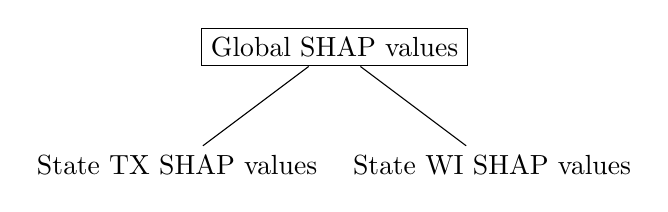
\begin{tikzpicture}
            [level 1/.style={sibling distance=40mm},
                level 2/.style={sibling distance=15mm}]
                \node[rectangle,draw] {Global SHAP values}
                child {node {State TX SHAP values} }
                child {node {State WI SHAP values}};
            \end{tikzpicture}
            \caption{State level SHAP values}
        \end{subfigure}%
        \vskip\baselineskip
        \begin{subfigure}{\textwidth}
            \centering
            \includegraphics[width=\linewidth]{sections/img/state_product}
            \caption{State level SHAP values}
            \label{fig:sub2}
        \end{subfigure}%
    \end{minipage}%
    \hfill
    \begin{minipage}{.45\textwidth}
        \centering
        \begin{subfigure}{\textwidth}
            \centering
            \includegraphics[width=\linewidth]{sections/img/state_tx_violin}
            \caption{TX state product SHAP summary}
            \label{fig:state_tx_violin_sub3}
        \end{subfigure}%
        \vskip\baselineskip
        \begin{subfigure}{\textwidth}
            \centering
            \includegraphics[width=\linewidth]{sections/img/state_wi_violin}
            \caption{WI state product SHAP summary}
            \label{fig:State_wi_violin_sub4}
        \end{subfigure}
    \end{minipage}
\end{figure}
%############################################################

%\subsection{State and product grouping}\label{subsec:state_prod_shap}
% TODO: The first lag value almost every time positively affects the forecast
\begin{figure}
    \centering
    \begin{minipage}{.45\textwidth}
        \centering
        \begin{subfigure}{\textwidth}
            \centering
            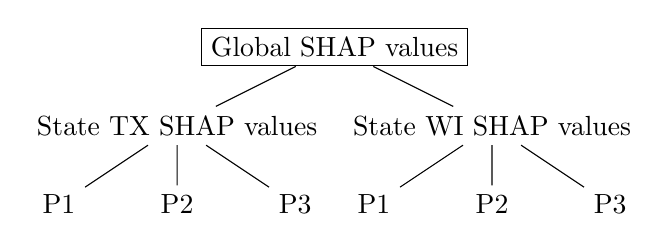
\begin{tikzpicture}
            [level 1/.style={sibling distance=40mm, level distance=10mm},
                level 2/.style={sibling distance=15mm, level distance=10mm}]
                \node[rectangle,draw] {Global SHAP values}
                child {node {State TX SHAP values}
                child {node {P1}}
                child {node {P2}}
                child {node {P3}}
                }
                child {node {State WI SHAP values}
                child {node {P1}}
                child {node {P2}}
                child {node {P3}}
                };
            \end{tikzpicture}
            \caption{Aggregation levels}
        \end{subfigure}%
        \vskip\baselineskip
        \begin{subfigure}{\textwidth}
            \centering
            \includegraphics[width=\linewidth]{sections/img/bar_state_product}
            \caption{State and product level SHAP values}
            \label{fig:state_product_sub2}
        \end{subfigure}%
    \end{minipage}%
    \hfill
    \begin{minipage}{.45\textwidth}
        \centering
        \begin{subfigure}{\textwidth}
            \centering
            \includegraphics[width=\linewidth]{sections/img/state_product_violin_1}
            \caption{TX state FOODS\_3\_586 product SHAP summary}
            \label{fig:state_prod_sub3}
        \end{subfigure}%
        \vskip\baselineskip
        \begin{subfigure}{\textwidth}
            \centering
            \includegraphics[width=\linewidth]{sections/img/state_product_violin2}
            \caption{WI state FOODS\_3\_080 product SHAP summary}
            \label{fig:state_prod_violin_sub4}
        \end{subfigure}
    \end{minipage}
    \caption{State and product level summary}
\end{figure}
%\begin{figure}
%    \centering
%%    \begin{tabular}{ c c }
%    \begin{subfigure}{.5\textwidth}
%        \centering
%        \begin{tikzpicture}
%        [level 1/.style={sibling distance=40mm, level distance=10mm},
%            level 2/.style={sibling distance=15mm, level distance=10mm}]
%            \node[rectangle,draw] {Global SHAP values}
%            child {node {State TX SHAP values}
%            child {node {P1}}
%            child {node {P2}}
%            child {node {P3}}
%            }
%            child {node {State WI SHAP values}
%            child {node {P1}}
%            child {node {P2}}
%            child {node {P3}}
%            };
%        \end{tikzpicture}
%        \caption{Aggregation levels}
%    \end{subfigure}%
%%    \vskip   \baselineskip
%    \begin{subfigure}{.5\textwidth}
%        \centering
%        \includegraphics[width=\linewidth]{sections/img/bar_state_product}
%        \caption{State and product level SHAP values}
%        \label{fig:state_product_sub2}
%    \end{subfigure}%
%    \hskip  % \baselineskip
%    \begin{subfigure}{.5\textwidth}
%        \centering
%        \includegraphics[width=\linewidth]{sections/img/state_product_violin_1}
%        \caption{TX state FOODS\_3\_586 product SHAP summary}
%        \label{fig:state_prod_sub3}
%    \end{subfigure}  %
%    \begin{subfigure}{.5\textwidth}
%        \centering
%        \includegraphics[width=\linewidth]{sections/img/state_product_violin2}
%        \caption{WI state FOODS\_3\_080 product SHAP summary}
%        \label{fig:state_prod_violin_sub4}
%    \end{subfigure}
%    \caption{State and product level summary}
%%    \end{tabular}
%\end{figure}



%%%%%%%%%%%%%%%%%%%%%%%%%%%%%%%%%%%%%%%%%%%%%%%%%%%%%%%%%%%%

% Store and product level
On the lowest level of the hierarchy presented in Figure \ref{fig:store_product_summary},
deviations can be revealed in the order of importance of the features.
For example, in Figure \ref{fig:store_prod_violin_sub4e} the week-of-year feature has a greater impact
on the forecast than some of the lag values that occurred in other cases in Figure \ref{fig:store_prod_sub3}.
This can be due to the fact that the store TX\_2 has a different seasonality pattern or
might have recurring special events, since the number of events is also a feature with higher impact on this store.
What is problematic in this case is that, due to the large number of series,
representation of the mean absolute SHAP value is hardly comprehensible in the previous form of the bar plot.
As a workaround, the grouping of feature contribution of each group is presented in Figure \ref{fig:store_product_sub2}.
What can be misleading in this case is the lack of order by impact and a different scale of the $x$ axis for each feature.

\begin{figure}
    \centering
    \begin{subfigure}{\textwidth}
        \centering
        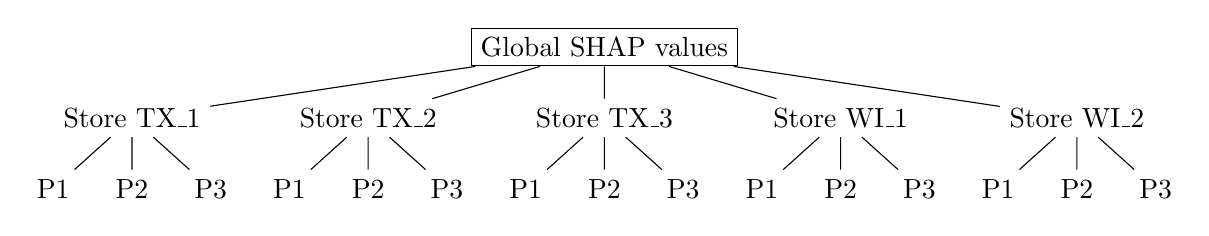
\begin{tikzpicture}
        [level 1/.style={sibling distance=30mm, level distance=9mm},
            level 2/.style={sibling distance=10mm,  level distance=9mm},]
%            level 3/.style={sibling distance=10mm}]
            \node[rectangle,draw] {Global SHAP values}
%            child {node {State TX}
            child {node {Store TX\_1}
            child {node {P1}}
            child {node {P2}}
            child {node {P3}}
            }
            child {node {Store TX\_2}
            child {node {P1}}
            child {node {P2}}
            child {node {P3}}
            }
            child {node {Store TX\_3}
            child {node {P1}}
            child {node {P2}}
            child {node {P3}}
            }
%            }
%            child {node {State WI}
            child {node {Store WI\_1}
            child {node {P1}}
            child {node {P2}}
            child {node {P3}}
            }
            child {node {Store WI\_2}
            child {node {P1}}
            child {node {P2}}
            child {node {P3}}
            };
        \end{tikzpicture}
        \caption{Aggregation levels}
    \end{subfigure}%
    \vskip\baselineskip
    \begin{subfigure}{.9\linewidth}
        \centering
     %  \includegraphics[width=0.8\linewidth, trim={0 67cm 30cm 0},clip ]{sections/img/store_product_shap2}
      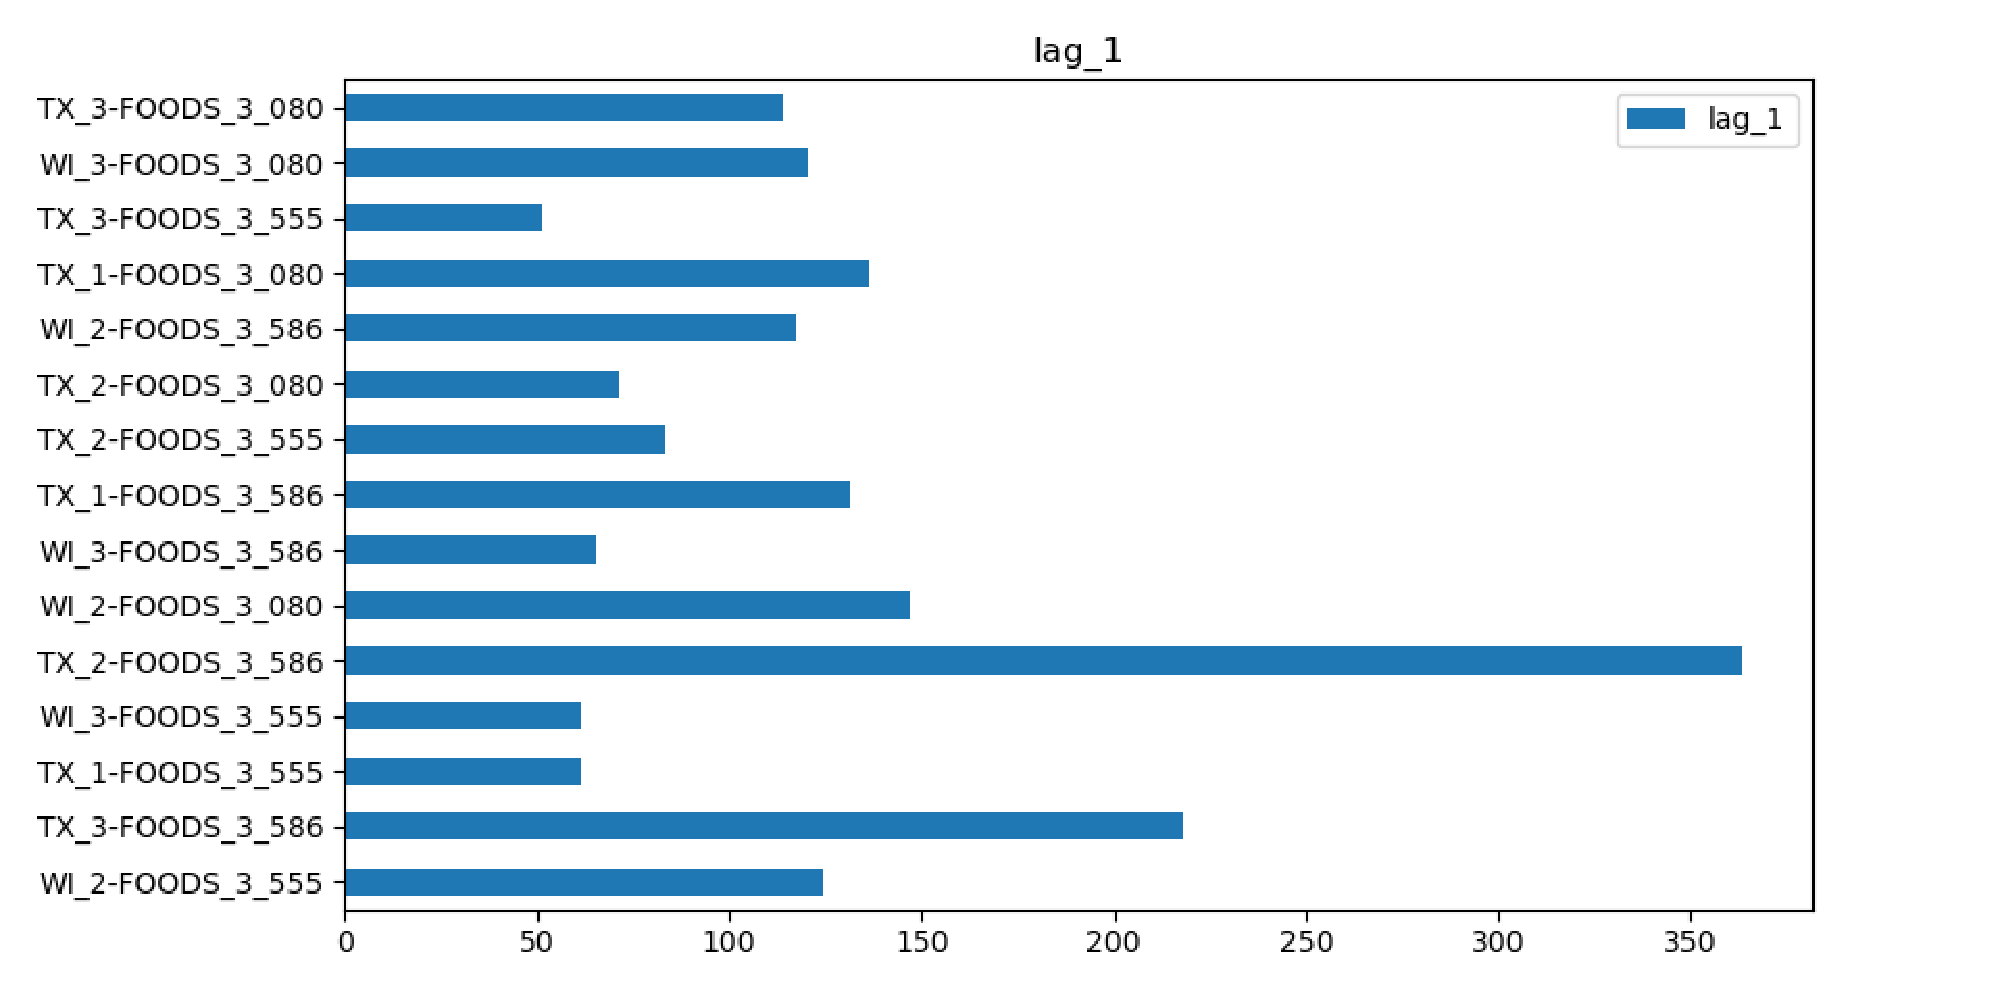
\includegraphics[width=0.8\linewidth]{sections/img/store_product_shap_2.eps}
        \caption{Store and product level SHAP values for one feature}
        \label{fig:store_product_sub2}
    \end{subfigure}%
    \vskip\baselineskip
    \begin{subfigure}{.5\textwidth}
        \centering
        \includegraphics[width=\linewidth,]{sections/img/store_product_violin3}
        \caption{Store TX\_3 FOODS\_3\_586 product SHAP summary}
        \label{fig:store_prod_sub3}
    \end{subfigure}%
    \begin{subfigure}{.5\textwidth}
        \centering
        \includegraphics[width=\linewidth]{sections/img/store_productviolin2}
        \caption{Store TX\_2 FOODS\_3\_080 product SHAP summary}
        \label{fig:store_prod_violin_sub4e}
    \end{subfigure}
    \caption{Store and product level summary}\label{fig:store_product_summary}
\end{figure}





    \section{Discussion}\label{sec:discussion}

%    \begin{itemize}
%        \item Provide a concise summary of the most important results from your analysis.
%        \item Relate the findings back to your research questions or hypotheses.
%        \item Highlight any unexpected or novel results.
%    \end{itemize}
%   \item \textbf{RQ1:} Can existing feature importance techniques be applied to multi-series and hierarchical models?


%\textcolor{red}{ TODO: Add discussion on the results and the implications for the research.}
%\textcolor{blue}{
%
%    \subsection*{Summary of Key Findings}
%    \begin{itemize}
%        \item Provide a concise summary of the most important results from your analysis.
%        \item Relate the findings back to your research questions or hypotheses.
%        \item Highlight any unexpected or novel results.
%    \end{itemize}
%    \subsection*{2. Interpretation of Results}
%    \begin{itemize}
%        \item Explain what the results mean in the context of your research objectives.
%        \item Relate your findings to the existing literature, showing how your work supports, extends, or challenges previous research.
%        \item Discuss the practical or theoretical significance of your findings. How do they contribute to the field?
%    \end{itemize}
%    \subsection*{3. Comparison with Previous Work}
%    \begin{itemize}
%        \item Compare your findings with those from other studies. Are your results consistent or different? Why might that be?
%        \item Discuss how your work fits into the broader literature and theoretical framework.
%    \end{itemize}
%    \subsection*{4. Implications of the Findings}
%    \begin{itemize}
%        \item Explain the practical or theoretical implications of your results.
%        \item Consider the broader impact of your findings on the field or on real-world applications.
%        \item If relevant, discuss policy or decision-making implications.
%    \end{itemize}
%    \subsection*{5. Limitations of the Study}
%    \begin{itemize}
%        \item Acknowledge any limitations in your research, such as constraints related to the methodology, data, or scope of the study.
%        \item Discuss how these limitations might have affected your results or interpretations.
%        \item Suggest ways these limitations could be addressed in future research.
%    \end{itemize}
%    \subsection*{6. Future Research Directions}
%    \begin{itemize}
%        \item Propose areas for future research based on your findings and the limitations you've identified.
%        \item Discuss how future studies could build on your work, including new methods, expanded datasets, or different research contexts.
%    \end{itemize}
%    \subsection*{7. Practical Applications (if applicable)}
%    \begin{itemize}
%        \item If your research has practical applications, discuss how your findings can be applied in industry, policy, or other fields.
%        \item Describe specific use cases or real-world scenarios where your work could be impactful.
%    \end{itemize}
%}

%\subsection{Expected contributions}
%
%This research is expected to contribute to the following areas:
%\begin{itemize}
%    \item Evaluation of method: Assessment of feature importance methods in hierarchical forecasting models.
%    \item Guidelines, best practices and limitations: Recommendations for explaining hierarchical forecasting models.
%    \item Tool development: Development of tools for better understanding of hierarchical models.
%\end{itemize}
%\subsection{Challenges and next steps} \label{subsec:challenges_next_steps}
%We already faced some challenges during the implementation of initial approach:
%\begin{itemize}
%    \item Proper tooling: SHAP library doesn't support models with categorical variables.
%    This is a limitation for the current library.
%    \item Visualizing the results: The SHAP library provides plotting functions, but for large number of series the plots were not working properly.
%\end{itemize}


%    \begin{itemize}
%        \item Acknowledge any limitations in your research, such as constraints related to the methodology, data, or scope of the study.
%        \item Discuss how these limitations might have affected your results or interpretations.
%        \item Suggest ways these limitations could be addressed in future research.
%    \end{itemize}


In this work, we managed to calculate the Shapley values for the predictions of a hierarchical forecasting model
with some limitations, while we also aggregated these values to different levels of the hierarchy.
By this we addressed the first two research questions.
We used a sample of a real-world dataset to evaluate the proposed method working towards the third research question.
We visualised the SHAP values at different levels of the hierarchy and provided some interpretation of the results.
To respond to the fourth research question, we plan to expand the literature review to include a wider range of XAI techniques.


%methodological limitations
This research is expected to contribute in several key areas.
First, it will provide an evaluation of feature importance methods in the context of hierarchical forecasting models.
This will help to identify what methods are most effective and how they can be applied to improve model interpretability.
Second, it aims to provide guidelines, best practices, and limitations of effectively explaining these models.
Finally, the research will support the development of tools that improve the understanding of hierarchical forecasting models
and their underlying rules and reasoning.


The limitations of our study include the handling of categorical variables in the SHAP library.
The effect of ordinal encoding that induces an order on the categorical variables may not be appropriate for all cases.
Low feature importance for the categorical variables may be due to the encoding method.
Recent research \cite{kristin_blesch_conditional_2023} proposes a method to handle categorical variables for conditional feature importance.
% data limitations
With regard to data limitations, the dataset used is simplified in multiple dimensions.
First, with aggregation of sales data at the weekly level, multiple exogenous variables such as special events could not be included.
Second, the dataset is limited to a single product category, which may not be representative of all hierarchical forecast scenarios.
Lastly, the input data was limited to the sales lag of the product without considering other products in the same category.
The independence of products in the same category may not be a realistic assumption.

During the implementation of our initial approach, we encountered several challenges.
One of the main issues was the lack of appropriate tools.
For example, the SHAP library does not support categorical features in the current version.
In addition,we faced difficulties in visualising the results;
although the SHAP library offers integrated graphing functions, these have not been effectively used to deal with
a large number of cohors, leading to errors and incomplete plots.
Although these issues are not straightforward to solve, they are a sign of unexplored areas in the field of XAI and hierarchical forecasting.

There are also potential risks that could impact research in addition to challenges.
One of the main risks is the availability of data, especially real-world datasets that include exogenous variables or demand drivers.
Synthetic datasets can be used as an alternative, but they may not capture the complexity of real-world scenarios.
The evaluation of methods is another potential risk, as it may be difficult to assess the performance of the explanation methods.
In case of application grounded evaluation, it may be difficult to find experts in the field who can provide meaningful feedback
given that each product category may require different domain knowledge\cite{doshi}.

\subsection{Future work} \label{subsec:future_work}

To address the challenges and limitations of the current research, several next steps are proposed for each part of the research.
\begin{itemize}
    \item First, the literature review will be extended to include a broader range of XAI techniques.
    Given the current context, we focus on feature importance-based evaluation, partial dependence plots, feature interaction, and other XAI techniques that should be included in the review.
    \item Data collection will be expanded to include synthetic datasets and additional real-world datasets.
    In addition, including more data from the actual dataset and forecasting on the day level can be a future direction.
    \item Evaluation and implementation of the tool for other methods will be needed.
    Conditional permutation importance can be also evaluated after implementing the method.
    \item The model implementation could be extended to include additional ML models for hierarchical forecasting.
    An additional enhancement to that would be dependent multiseries forecasting, as usually product sales are not independent
of each other, especially in the same product category.
    \item Rule extraction based on feature importance and interaction can be a future direction.
    \item After covering the methodological aspects, an empirical study with evaluation in terms of accuracy and computational efficiency is planned.
\end{itemize}


%\textbf{Next steps}
%\begin{itemize}
%%    \item Literature Review: Extend it with focus on the following aspects:
%%        \begin{itemize}
%%            \item XAI(Explainable AI) techniques and their application in demand forecasting.
%%            \item Application of other XAI methods in hierarchical and multi-series models.
%%            \item Feature importance and model reasoning in hierarchical models.
%%            \item Challenges and limitations of existing XAI methods.
%%        \end{itemize}
%%    \item Data collection: Create synthetic dataset and collect additional real-world datasets for hierarchical demand forecasting.
%%    \item Tool evaluation or implementation: Evaluate existing libraries for hierarchical forecasting and XAI techniques or implement custom tools specialized for hierarchical forecasting.
%%    \item Model implementation: Train and evaluate additional ML models for hierarchical forecasting.
%    \item Feature importance analysis: Apply XAI techniques to determine feature importance and assess their impact on forecasts.
%    \item Model reasoning: Analyze feature contributions to uncover underlying rules, especially at different hierarchy levels, and how to extract rules.
%    Synthesize the results to provide a better understanding of the model's reasoning
%
%\end{itemize}

%For future work we plan to conduct an empirical study on the applicability of feature importance methods to hierarchical forecasting models.
%For this purpose we plan to use both synthetic and real-world datasets to evaluate the methods.
%Additionally, the inclusion fo these techniques in decision support systems can be a future direction.

%\textcolor{red}{
%
%    \subsection{Conclusion}
%    \begin{itemize}
%        \item Summary of objectives and findings.
%        \item Importance of XAI in improving hierarchical forecasting models and understanding their reasoning.
%    \end{itemize}
%}

\subsection{Conclusion}\label{subsec:conclusion}
Nowadays every organisation thrives in the direction of becoming data driven.
In this context, data-driven decision making is crucial for optimising business processes to remain competitive.
This effort is supported by the use of data mining, machine learning, and AI techniques.
To avoid blindly trusting ML models,it is crucial to understand the reasoning behind their decisions.
Our goal is to demystify hierarchical forecasting models by applying XAI techniques.

This study explores the usage of SHAP values to explain the importance of features in hierarchical forecasting models.
Our preliminary results focused on the practical aspects of aggregating SHAP values at different levels of
hierarchy. This approach provides insights into the model's reasoning.
We plan to extend this work by evaluating other XAI techniques to enhance the explainability of hierarchical forecasting models.


\textbf{Acknowledgement}

This work was done in collaboration with my Ph.D. supervisor, Laura Diosan, from Babes-Bolyai University.
I am grateful for her continued support and encouragement throughout this research.






%
\section{Research plan} \label{sec:research_plan}
This section outlines the approach to be taken to continue the research and achieve the expected contributions.

Our plan includes the following stages:

\textbf{1. Literature Review}

Extend the literature review with focus on the following aspects:
\begin{itemize}
    \item XAI(Explainable AI) techniques and their application in demand forecasting.
    \item Hierarchical time-series forecasting models and their importance in demand forecasting.
    \item Application of feature importance methods in hierarchical and multi-series models.
    \item Feature importance and model reasoning in hierarchical models.
    \item Challenges and limitations of existing XAI methods.
\end{itemize}

\textbf{2. Research methodology}

\begin{itemize}
    \item Data collection: Create synthetic dataset and collect additional real-world datasets for hierarchical demand forecasting.
    \item Tool evaluation: Evaluate existing libraries for hierarchical forecasting and XAI techniques.
    \item Model implementation: Train and evaluate additional ML models for hierarchical forecasting.
    \item Feature importance analysis: Apply XAI techniques to determine feature importance and assess their impact on forecasts.
    \item Model reasoning: Analyze feature contributions to uncover underlying rules, especially at different hierarchy levels.
    \item Conduct empirical study with evaluation in terms of accuracy and computational efficiency.
\end{itemize}







%%
%% Define the bibliography file to be used
    \bibliography{sample-ceur}

%%
%% If your work has an appendix, this is the place to put it.
    \appendix

%\section{Online Resources}
%
%
%The sources for the ceur-art style are available via
%\begin{itemize}
%\item \href{https://github.com/yamadharma/ceurart}{GitHub},
%% \item \href{https://www.overleaf.com/project/5e76702c4acae70001d3bc87}{Overleaf},
%\item
%  \href{https://www.overleaf.com/latex/templates/template-for-submissions-to-ceur-workshop-proceedings-ceur-ws-dot-org/pkfscdkgkhcq}{Overleaf
%    template}.
%\end{itemize}

\end{document}

%%
%% End of file
